\section{Auswertung}
\label{sec:Auswertung}
In den folgenden Tabellen sind die gemessenen Werte zusammenfassend dargestellt.

\begin{table}[H]
  \centering
  \caption{Die Messwerte der Reflexion an einem Spiegel für verschiedene Winkel. Verwendet wurde der grüne Laser mit $\lambda = \SI{532}{\nano\meter}$.}
  \label{tab:MessungAufgabe1}
  \sisetup{table-format=2.1}
  \begin{tabular}{S S}
    \toprule
    {Einfallswinkel[\si{\degree}]} & {Ausfallswinkel[\si{\degree}]} \\
    \midrule
    69   &  69   \\
    42   &  43   \\
    30.5 & 30.5  \\
    55   & 56    \\
    72   & 72    \\
    20   & 20    \\
    35   & 35    \\
    52   & 52.5  \\
    \bottomrule
  \end{tabular}
\end{table}

\begin{table}[H]
  \centering
  \caption{Die Messwerte der Brechung an einer planparallelen Platte der Messung 1 für verschiedene Winkel. Verwendet wurde der grüne Laser mit $\lambda = \SI{532}{\nano\meter}$.}
  \label{tab:MessungAufgabe2}
  \sisetup{table-format=2.2}
  \begin{tabular}{S S}
    \toprule
    {Einfallswinkel[\si{\degree}]} & {Brechungswinkel[\si{\degree}]} \\
    \midrule
    69 & 39    \\
     0 &  0    \\
    10 &  7    \\
    30 & 20    \\
    40 & 25.5  \\
    75 & 40.5  \\
    55 & 33.5  \\
    38 & 24.25 \\
    \bottomrule
  \end{tabular}
\end{table}

\begin{table}[H]
  \centering
  \caption{Die Messwerte der Brechung an einer planparallelen Platte der Messung 2 für verschiedene Winkel. Verwendet wurde der grüne Laser mit $\lambda = \SI{532}{\nano\meter}$.}
  \label{tab:MessungAufgabe3}
  \sisetup{table-format=2.1}
  \begin{tabular}{S S}
    \toprule
    {Einfallswinkel[\si{\degree}]} & {Brechungswinkel[\si{\degree}]} \\
    \midrule
    0  &  0     \\
   45  & 28.5   \\
   60  & 36     \\
   20  & 13.5   \\
   51  & 31.5   \\
    3  &  3.5   \\
    \bottomrule
  \end{tabular}
\end{table}

\begin{table}[H]
  \centering
  \caption{Die Messwerte der Brechung an einem Prisma für verschiedene Winkel. Verwendet wurde der grüne Laser mit $\lambda = \SI{532}{\nano\meter}$ und der rote Laser mit $\lambda = \SI{635}{\nano\meter}$.}
  \label{tab:MessungAufgabe4}
  \sisetup{table-format=2.1}
  \begin{tabular}{S S S}
    \toprule
    {Einfallswinkel[\si{\degree}]} & {Ausfallswinkel $L_{Gruen}$[\si{\degree}]} & {Ausfallswinkel $L_{Rot}$[\si{\degree}]} \\
    \midrule
    30  & 82   & 84   \\
    35  & 73.5 & 74.5 \\
    39  & 60   & 60.7 \\
    46  & 48   & 49.5 \\
    60  & 42   & 43   \\
    \bottomrule
  \end{tabular}
\end{table}

\begin{table}[H]
  \centering
  \caption{Die gemessenen Beugungsmaxima der Beugung an einem Strichgitter mit 600 Linien/mm. Verwendet wurde der grüne Laser mit $\lambda = \SI{532}{\nano\meter}$.}
  \label{tab:MessungAufgabe51}
  \sisetup{table-format=2.1}
  \begin{tabular}{S S S }
    \toprule
    {Laserposition[\si{\degree}]} & $B_{max1,2}$[\si{\degree}] & $B_{max3}$[\si{\degree}]\\
    \midrule
    0  & \pm 22.5 & 0 \\
    \bottomrule
  \end{tabular}
\end{table}

\begin{table}[H]
  \centering
  \caption{Die gemessenen Beugungsmaxima der Beugung an einem Strichgitter mit 300 Linien/mm.}
  \label{tab:MessungAufgabe52}
  \sisetup{table-format=2.1}
  \begin{tabular}{S S S S}
    \toprule
    {Laserposition[\si{\degree}]} & $B_{max1,2}$[\si{\degree}] & $B_{max3,4}$[\si{\degree}] & $B_{max5}$[\si{\degree}]\\
    \midrule
    0 & \pm 22 & \pm 10.7 & 0 \\
    \bottomrule
  \end{tabular}
\end{table}

\begin{table}[H]
  \centering
  \caption{Die gemessenen Beugungsmaxima der Beugung an einem Strichgitter mit 100 Linien/mm.}
  \label{tab:MessungAufgabe53}
  \sisetup{table-format=2.1}
  \begin{tabular}{S S S S S S S S S}
    \toprule
    {Laserposition[\si{\degree}]} & $B_{1,2}$[\si{\degree}] & $B_{3,4}$[\si{\degree}] & $B_{5,6}$[\si{\degree}] & $B_{7,8}$[\si{\degree}] & $B_{9,10}$[\si{\degree}] & $B_{11,12}$[\si{\degree}]  & $B_{13,14}$[\si{\degree}] & $B_{15}$[\si{\degree}]\\
    \midrule
    0 & \pm 26 & \pm 22 & \pm 18 & \pm 14 & \pm 11 & \pm 7.2 & \pm 3.7 & 0 \\
    \bottomrule
  \end{tabular}
\end{table}

\subsection{Reflexion}
\label{sec:reflexionauswertung}
Die Ergebnisse der Untersuchung der Reflexion sind in Tabelle \ref{tab:MessungAufgabe1} abgebildet. Die maximale Genauigkeit der Messung liegt ungefähr bei einem Grad, da die Skalen, von denen abgelesen wurden, keine kleineren Unterteilungen besaßen. Nach dem Reflexionsgesetz
\eqref{eqn:reflexion} beträgt die maximale Abweichung der Messung von der Theorie $\pm \SI{1}{\degree}$.
In der folgenden Abbildung sind der Einfallswinkel und der Reflexionswinkel gegeneinander aufgetragen.

\begin{figure}[H]
  \centering
  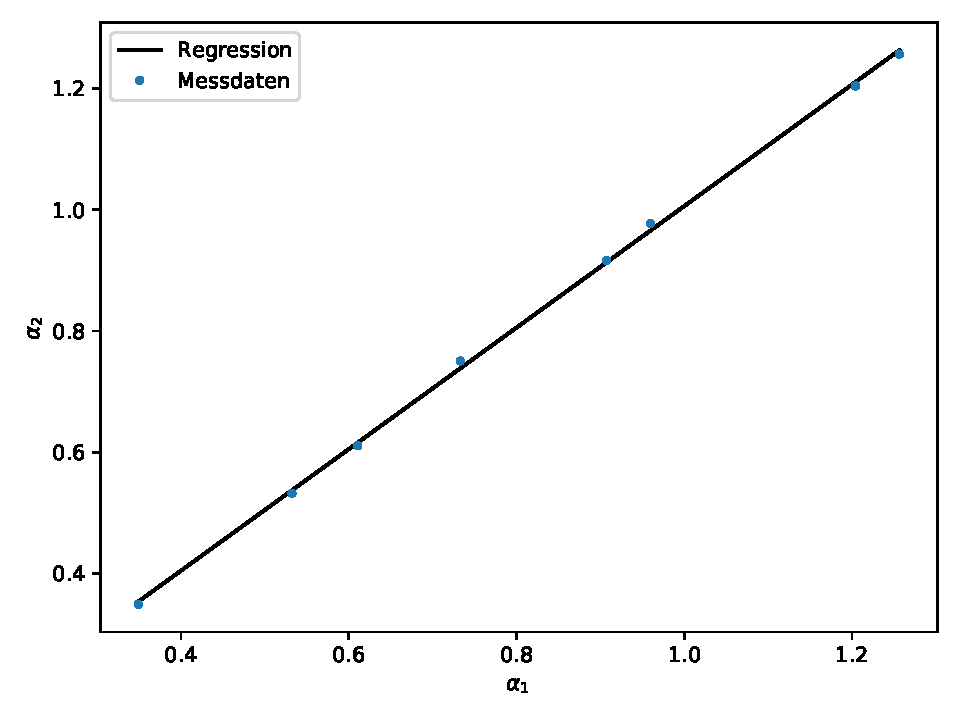
\includegraphics[scale= 0.7]{auswertung/plot1.pdf}
  \caption{Einfallswinkel $\alpha_1$ und Reflexionswinkel $\alpha_2$.}
  \label{fig:plot1}
\end{figure}

\subsection{Brechung}
\label{sec:brechungauswertung}
Die bestimmten Brechungswinkel sind in Tabelle \ref{tab:MessungAufgabe2} abgebildet.
Der Brechungsindex, berechnet nach dem Brechungsgesetz \eqref{eqn:brechung2} unter Zuhilfenahme von \textit{numpy}\cite{numpy},
beträgt
\begin{equation*}
  n = 1.476 \pm 0.010.
  \label{eqn:brechungsindexausw}
\end{equation*}
In folgender Grafik sind die berechneten Brechungsindizes für verschiedene Winkel angegeben.
\begin{figure}[H]
  \centering
  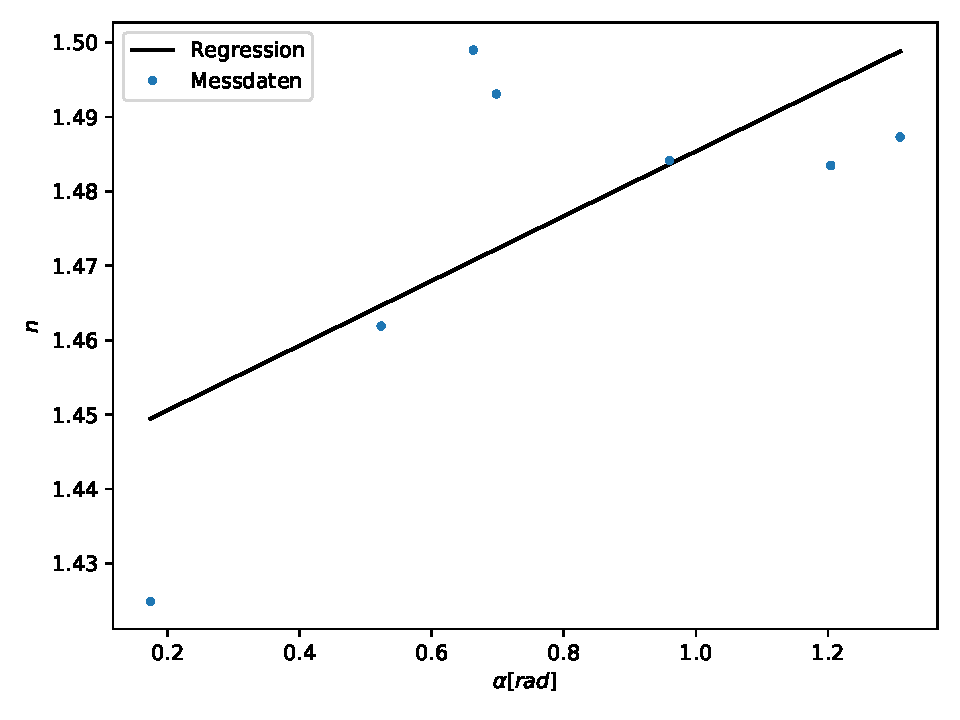
\includegraphics[scale=0.7]{auswertung/plot2.pdf}
  \caption{Die berechneten Brechungsindizes beim jeweiligen Einfallswinkel.}
  \label{fig:plot2ausw}
\end{figure}
\noindent
Die Literaturwerte für den Brechungsindex sind in Tabelle \ref{tab:brechungsind} angegeben.
Es ergibt sich eine prozentuale Abweichung des berechneten Wertes von dem Literaturwert von
\begin{equation*}
  p = 1.1 \pm 0.6 \si{\percent}.
  \label{eqn:abweichung}
\end{equation*}
Für die Lichtgeschwindigkeit in Plexiglas ergibt sich dann mit Gleichung \ref{eqn:brechung1}
\begin{equation*}
  v=(2.031 \pm 0.013) \cdot 10^8 \si{\meter\per\second}.
  \label{eqn:lichtgeschwausw}
\end{equation*}

\subsection{Planparalle Platten}
\label{sec:planplatteauswertung}
Die gemessenen Einfalls- und Brechungswinkel sind in Tabelle \ref{tab:MessungAufgabe3} dargestellt. Der Strahlversatz wurde auf zweierlei Arten ermittelt: einmal unter Verwendung des gemessenen Einfalls- und Brechungswinkels, sowie einmal unter Verwendung des gemessenen Einfallswinkels und des mit dem Brechungsgesetz berechneten Brechungswinkels.
Beide Ergebnisse sind in Abbildung \ref{fig:plot3ausw} dargestellt.
\begin{figure}[H]
  \centering
  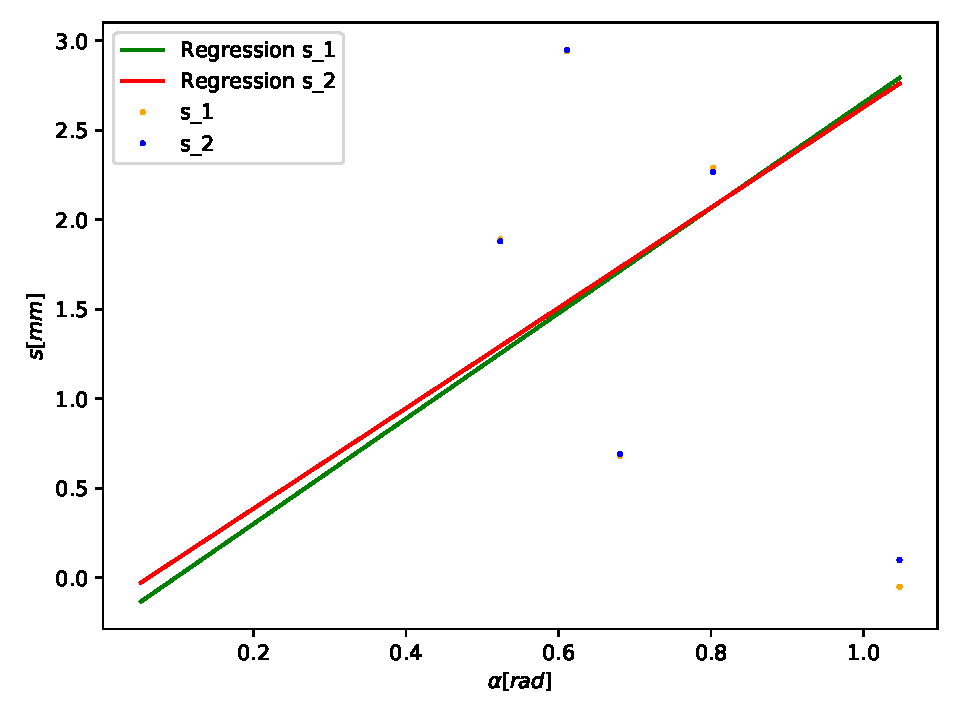
\includegraphics[scale=0.7]{auswertung/plot3.pdf}
  \caption{Die berechneten Strahenversätze beim jeweiligen Einfallswinkel.}
  \label{fig:plot3ausw}
\end{figure}
\noindent
Hierbei bezeichnet $s_1$ die Berechnung des Strahlversatzes auf Basis der Messung beider Winkel und $s_2$ die Berechnung auf Basis des Einfallswinkels und des Brechungsgesetzes.
Die Werte sind in folgender Tabelle mit der prozentualen Abweichung voneinander aufgeführt.

\begin{table}[H]
  \centering
  \caption{Werte für den Strahlversatz, mit zwei Methoden berechnet.}
  \label{tab:strahlversatzausw}
  \sisetup{table-format=3.3}
  \begin{tabular}
    {S S S S}
    \toprule
    {$\alpha [\si{\degree}]$} & {$s_1 [\si{\meter}]$} & {$s_2 [\si{\meter}]$} & {Abweichung $[\si{\percent}]$} \\
    \midrule
    45 & {$1.891 \cdot 10^{-3}$} & {$1.879 \cdot 10^{-3}$} & {$0.591$} \\
    60 & {$2.941 \cdot 10^{-3}$} & {$2.947 \cdot 10^{-3}$} & {$0.215$} \\
    20 & {$6.811 \cdot 10^{-4}$} & {$6.916 \cdot 10^{-4}$} & {$1.547$} \\
    51 & {$2.290 \cdot 10^{-3}$} & {$2.267 \cdot 10^{-3}$} & {$1.024$} \\
     3 & {$-5.115 \cdot 10^{-5}$} & {$9.893 \cdot 10^{-5}$} & {$293.4$} \\
    \bottomrule
  \end{tabular}
\end{table}
\noindent
Die Werte und Abweichung wurde unter Verwendung des Brechungsgesetzes \eqref{eqn:brechung1} sowie der Formel für den
Strahlversatz \eqref{eqn:strahlenversatz} mithilfe von \textit{numpy}\cite{numpy} berechnet.

\subsection{Prisma}
\label{sec:prismaauswertung}
Die Messergebnisse der Ein- und Ausfallswinkel sind in Tabelle \ref{tab:MessungAufgabe4} dargestellt. In folgender Abbildung ist der eingestellte Winkel des Lasers gegen die erfahrene Ablenkung des Lichtstrahls aufgetragen.
\begin{figure}[H]
  \centering
  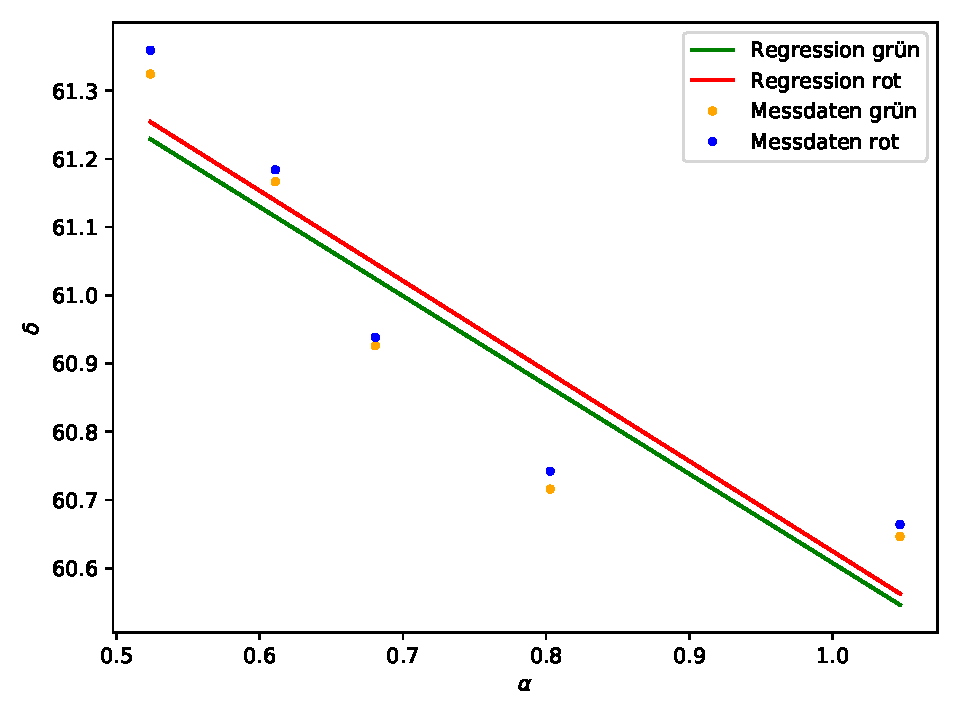
\includegraphics[scale=0.7]{auswertung/plot4.pdf}
  \caption{Der Ablenkwinkel beim jeweiligen Einfallswinkel.}
  \label{fig:plot4ausw}
\end{figure}
\noindent
Die Ablenkung wurde mit der Formel \eqref{eqn:ablenkwinkel} mit \textit{numpy}\cite{numpy} ermittelt. Der verwendete Brechungsindex beträgt $n = 1.61282$, siehe Tabelle \ref{tab:brechungsind}.


\subsection{Beugung am Gitter}
\label{sec:beugungauswertung}
In folgender Tabelle sind die berechneten Wellenlängen sowie die prozentuale Abweichung von dem Literaturwert $\lambda = \SI{635}{\nano\meter}$ aufgeführt.
\begin{table}[H]
  \centering
  \caption{Die aus der Beugung berechneten Wellenlängen.}
  \label{tab:wellenlausw}
  \sisetup{table-format=3.3}
  \begin{tabular}
    {S S S S S S}
    \toprule
    {$\lambda_{600} [\si{\nano\meter}]$} & $p_{600} [\si{\percent}]$ & {$\lambda_{300} [\si{\nano\meter}]$} & $p_{300} [\si{\percent}]$ & {$\lambda_{100} [\si{\nano\meter}$} & $p_{100} [\si{\percent}]$ \\
    \midrule
      0.0   &   100     &     0.0    &    100    &     0.0   &  100     \\
    318.903 &   49.779  &   309.444  &    51.269 &   322.662 &  49.187  \\
            &           &   416.230  &    34.452 &   417.777 &  34.208  \\
            &           &            &           &   477.022 &  24.878  \\
            &           &            &           &   483.844 &  23.804  \\
            &           &            &           &   515.028 &  18.893  \\
            &           &            &           &   535.152 &  15.724  \\
            &           &            &           &   547.964 &  13.706  \\
    \bottomrule
  \end{tabular}
\end{table}
\noindent
Die Wellenlängen wurden nach \eqref{eqn:gitterintmax} mittels \textit{numpy}\cite{numpy} berechnet. Hier konnte nur der grüne Laser mit $\lambda = \SI{635}{\nano\meter}$ verwendet werden, da nur dieser aufgrund der
Anordnung der Geräte auf das Gitter gerichtet werden konnte.
